\documentclass[tikz,border=10pt]{standalone}
\begin{document}
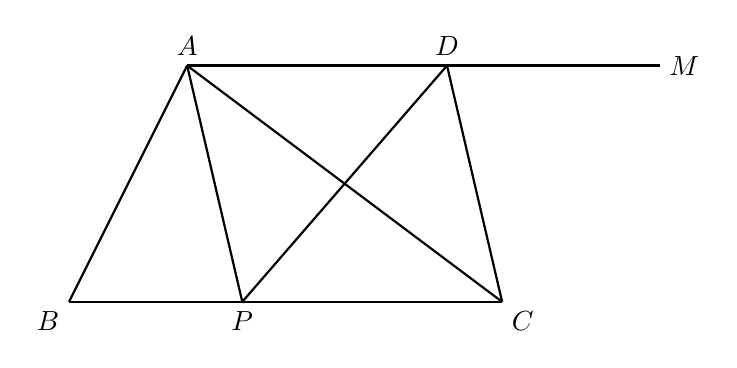
\begin{tikzpicture}
  \coordinate (A) at (1.5,3);
  \coordinate (B) at (0,0);
  \coordinate (C) at (5.5,0);
  \coordinate (D) at (4.8,3);
  \coordinate (P) at (2.2,0);
  \coordinate (M) at (7.5,3);

  \draw[thick] (B) -- (C);
  \draw[thick] (A) -- (D);
  \draw[thick] (D) -- (M);
  \draw[thick] (A) -- (B);
  \draw[thick] (D) -- (C);
  \draw[thick] (A) -- (P);
  \draw[thick] (A) -- (C);
  \draw[thick] (P) -- (D);

  \node[above] at (A) {$A$};
  \node[below left] at (B) {$B$};
  \node[below] at (P) {$P$};
  \node[below right] at (C) {$C$};
  \node[above] at (D) {$D$};
  \node[right] at (M) {$M$};
\end{tikzpicture}
\end{document}
